\begin{enumerate}[label=\thechapter.\arabic*,ref=\thechapter.\theenumi]
    \item The discrete-time Fourier transform of a signal x\sbrak{n} is $X\brak{\Omega}=\brak{1+\cos{\Omega}}e^{-j\Omega}$. Consider that $x_{p}\sbrak{n}$ is a periodic signal of period $N=5$ such that
        \begin{align}
            x_p\sbrak{n}&=x[n],\text{for n= 0, 1, 2}\\
            &=0,\text{for n= 3, 4}
        \end{align}
        Note that $x_p\sbrak{n}=\sum_{k=0}^{N-1}a_{k}e^{j\frac{2\pi}{N}kn}$. The magnitude of the Fourier series coefficient $a_3$ is \rule{3cm}{0.15mm} \brak{\text{Round off to 3 decimal places}}.\hfill(GATE EE 2023)
        \solution
        \newpage

\item Let a frequency modulated (FM) signal : $ x(t) = A \cos(\omega_c t + k_f \int_{-\infty}^{t} m(\lambda) d\lambda)$ , where $ m(t) $is a message signal of bandwidth $ W $. It is passed through a non-linear system with output $y(t) = 2x(t) + 5(x(t))^2 $.
Let $B_T $denote the FM bandwidth. The minimum value of $ \omega_c $ required to recover $ x(t) $ from $ y(t) $ is:\\
\begin{enumerate}[label = (\Alph*)]
\item $B_T + W$ \\
\item $\dfrac{3}{2} B_T$ \\
\item $2B_T + W$ \\
\item $\dfrac{5}{2} B_T$ \\
\end{enumerate}

\solution
\newpage

\item Let an input $x[n]$ having discrete-time Fourier transform
$X(e^{j\Omega}) = 1 - e^{-j\Omega} + 2e^{-3j\Omega}$
be passed through an LTI system. The frequency response of the LTI system is 
$H(e^{j\Omega}) = 1 - \frac{1}{2} e^{-2j\Omega}$
The output $y[n]$ of the system is \\ \hfill(GATE EC 2023)
\solution 
\newpage

\item Let $x_1(t) = u(t + 1.5) - u(t - 1.5)$ and $x_2(t)$ is shown in the figure below. For $y(t) = x_1(t) * x_2(t)$, the $\int_{-\infty}^{\infty} y(t) \, dt$ is \underline{\hspace{2cm}}.
\begin{figure}[htbp]
    \centering
    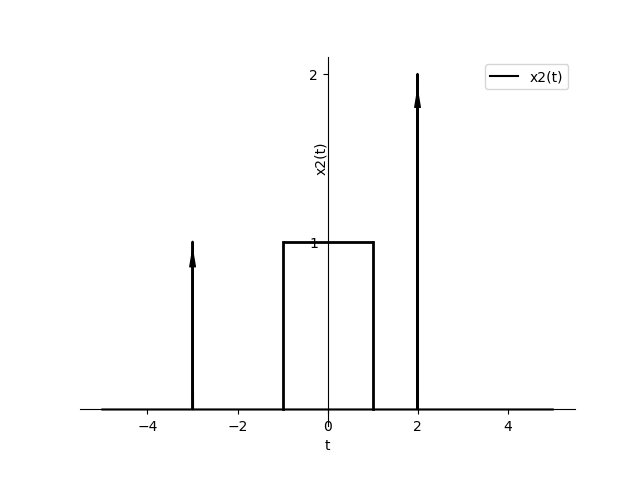
\includegraphics[width=0.5\textwidth]{2023/EC/58/figs/gatefig.png}
    \caption{Figure}
    \label{fig:graph}
\end{figure}

\hfill(GATE EE 2023) \\
\solution
\pagebreak
\end{enumerate}
